\cleardoublepage
\singlespacing
\chapter{EVALUATION \& RESULTS}
\label{c:evaluation}
\doublespacing\nointerlineskip

%Thwas chapter presents evaluation. The models and algorithms were
%tested extensively on benchmarks, which was described in
%section~\ref{s:benchmarks}, and the results were dwascussed in
%section~\ref{s:results}

In order to evaluate the performance of our fault tolerance primitive, we have
introduced some metrics to test how well it perform, and whether after node
failures requirements could still be met under small network.

\begin{enumerate}
\item Whether failover kickoff successfully after failure
\item Memory overhead for Strips
\item Message overhead for failure recovery, including reconfiguration
\item Time to detect and recover from failure
\end{enumerate}

We measured system performance live by collecting data from sensor nodes while
running. Sensor nodes were programmed to send out their tracking data to
a central data sink at appropriate times such as after node initialization or
when the failure was resolved.

The application, fault tolerance policy, network topology were described in the
following sections.


\section{Application}

Application shown in Figure~\ref{fig:fbp-application} will be deployed.  There
will be four components: 

\begin{enumerate}
\item Numeric Controller component represents a user input device which outputs
a number from 0 to 255. Light Sensor was a photodetector sensor which detects the
level of light intensity. 
\item Threshold component represents a conditional function which takes two
inputs, Threshold and Value, and, depending on the Operator attribute, return
true if the Operator was set to GT (Greater Than) and the Value was higher than
the Threshold value.
\item Light Actuator component represents a relay intercepting the power source for
a light bulb, it has a property OnOff which turns on the light if it was set to
true, otherwise the light will be turned off.
\item Light Sensor component represents a sensor sensing the light intensity in the surrounding
  area.
\end{enumerate}


\section{Policy}

The component fault tolerance policy for the application was set with the
following parameters:

\begin{description}
  \item[Numeric Controller component] \hfill \\
    Redundancy Level: 1\\
    Fault Detection Time: 2 sec\\
  \item[Light Sensor component] \hfill \\
    Redundancy Level: 2\\
    Fault Detection Time: 2 sec\\
  \item[Threshold component] \hfill \\
    Redundancy Level: 1\\
    Fault Detection Time: 2 sec\\
  \item[Light Actuator component] \hfill \\
    Redundancy Level: 9\\
    Fault Detection Time: 2 sec\\
\end{description}

Since we set timeout at 2 times of heartbeat period, assuming the worst time to detect
failure takes the full length of fault detection time, the heartbeat
period was therefore 1 sec, which was one half of the fault detection time.

\section{Heartbeat Protocol Arrangement}

We deployed 10 nodes in a room in our test lab, which results in a fully
connected network. Therefore only one heartbeat chain loop was formed.

The heartbeat procotol arrangement was simple. Every node was sending heartbeat to
previous node except the first node, which sends to the last. For example, node
1 receives heartbeat message from node 2, node 2 receives heartbeat message from
node 3, etc. Figure~\ref{fig:heartbeat-protocol-arrangement} illustrates the
arrangement for this experiment.

\begin{figure}[h!]
\centering
    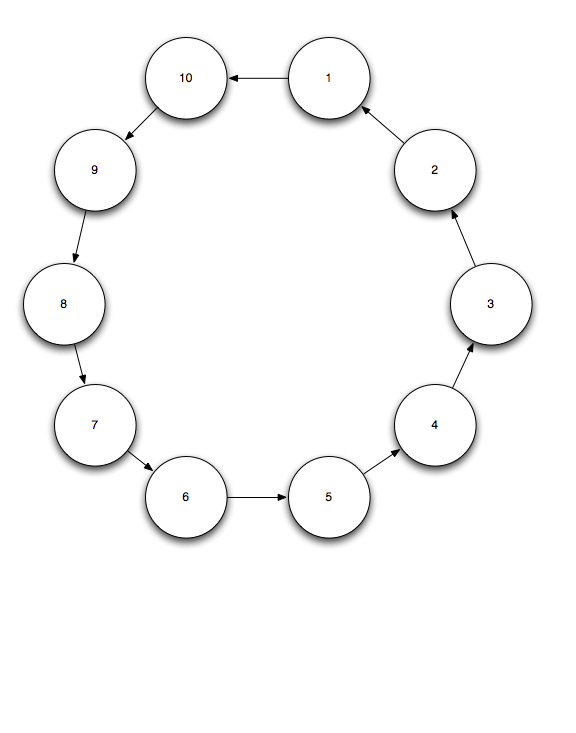
\includegraphics[width=\linewidth]{figures/heartbeat-protocol-arrangement}
\caption{Heartbeat protocol arrangement where the arrows indicate the direction
  heartbeat messages get sent to}
\label{fig:heartbeat-protocol-arrangement}
\end{figure}

\section{Hardware Platform}

All boards were equipped with an Atmel ATmega2560-16AU 8-bit microcontroller
with 4K of EEPROM and 64k of flash. The figure~\ref{fig:wudevice} showed the
board used in the experiments. The boards hardware design was based upon Arduino
hardware referenced design, in addition, every board has wires for mounting
multiple wireless protocol adapters supporting protocol standards such as
ZWave~\cite{ZWave}. ZWave is a wireless communication protocol designed for home
automation, specifically to remotely controlled applications in residential and
light commercial environments.

In the following experiment, every board was only equipped with a ZWave adapter
and only communicating wirelessly through the ZWave adapter.  Every board was
also pre-installed with “NanoKong”~\cite{Su}, which includes
NanoVM~\cite{Harbaum2006} and WuKong Profile Framework that supports all the
basic WuKong framework protocols including the new additions from the work in
the previous chapter. A PC with wireless access was dedicated for hosting the
WuKong Master software which was responsible for managing WuKong applications
for the whole system and serves as a mean to present an interface to the users.  

\begin{figure}[h!]
\centering
    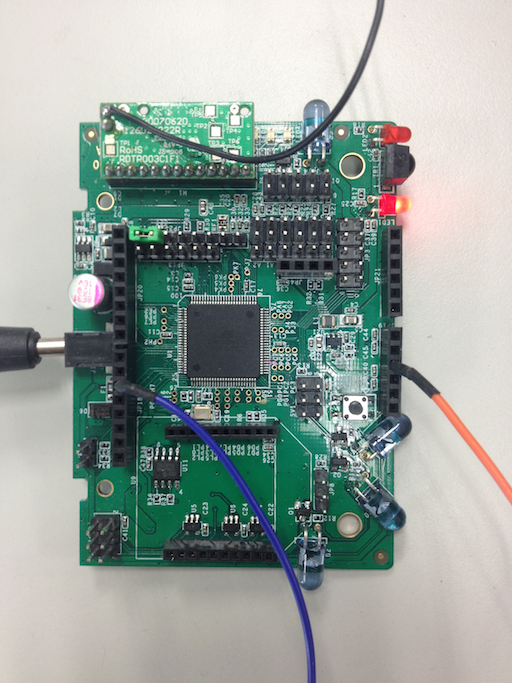
\includegraphics[width=\linewidth]{figures/wudevice}
\caption{An WuDevice equipped with ZWave radio on the top, and running
  a ATmega2560 8-bit microcontroller in the middle}
\label{fig:wudevice}
\end{figure}

\section{Experimental Setup}

%1(2)
%2(4)
%3(5)
%4(6)
%5(7)
%6(10)
%7(12)
%8(13)
%9(14)
%10(15)

\begin{table}
\centering
\caption{Node setup}
\label{tbl:setup}
  \begin{tabular}{|l|l|}
  \hline
  \textbf{Node Id} & \textbf{Equipped Resources} \\
  \hline
  1 & Light Actuator \\
  \hline
  2 & Numeric Controller, Threshold, Light Sensor \\
  \hline
  3 & Light Actuator \\
  \hline
  4 & Light Actuator \\
  \hline
  5 & Light Actuator, Light Sensor \\
  \hline
  6 & Light Actuator \\
  \hline
  7 & Light Actuator \\
  \hline
  8 & Light Actuator \\
  \hline
  9 & Light Actuator \\
  \hline
  10 & Light Actuator \\
  \hline
  \end{tabular}
\end{table}

\begin{figure}[h!]
  \centering
    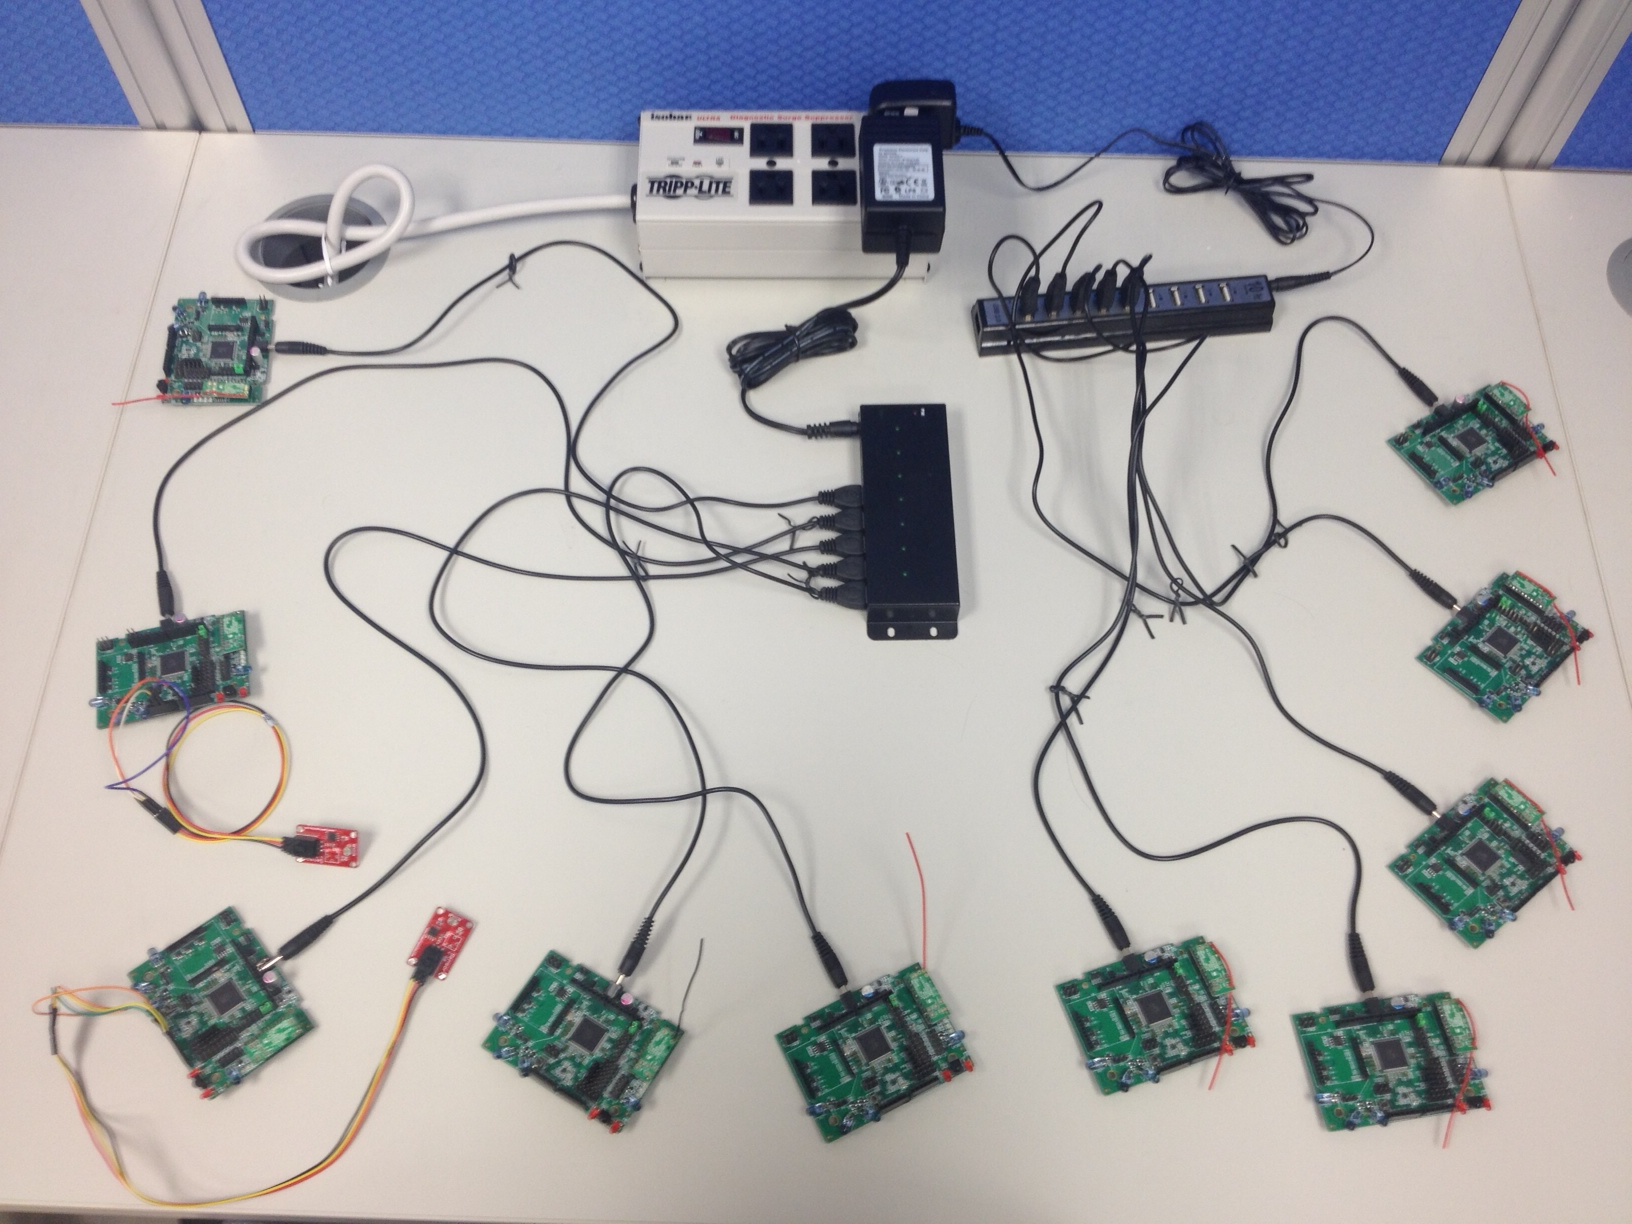
\includegraphics[width=\linewidth]{figures/system-setup}
    \caption{Whole system setup with ten nodes, two of them were equipped with light sensors}
  \label{fig:system-setup}
\end{figure}

The complete system setup is shown in figure~\ref{fig:system-setup}. Ten boards
were used in the experiments. Two of them were equipped with a Arduino brick
light sensor~\cite{brick} that returns light intensity value from 0 to 1023. The
rest were equipped with a onboard LED as a simple light source. Boards with
light sensor were assigned a light sensor component. Boards with light actuator
were assigned a light actuator component.  One of them were assigned a Numeric
Controller component, and Threshold component for the deployed application.
Every WuDevice would be able to talk to each other directly through ZWave
wireless adapter. The deployment formed a fully connected network. We simulated
a node failure by removing power supply from a WuDevice. The detail of each node
setup was shown in table~\ref{tbl:setup}.

\section{Mapping Results}

The result of the mapping and the strips were shown in
table~\ref{tbl:mapping-result}. Each row represented each component in the
application, where strips were ordered from the left. Numeric Controller was
mapped to only node 1; Light sensor was mapped to node 2 and 5, where 2 hold the
active WuObjects when deployed; Light actuator was mapped to 9 nodes, and node
1 hold the active WuObject when deployed; Threshold was mapped to node 2.  The
result indicated that the only active nodes were 2, and 1 right after deployment.

Table~\ref{tbl:results-memory-overhead-strip} listed the memory overhead of each
strip in the application. Each entry in the strip consumes 2 bytes, one byte for
addressing and the other is for internal addressing for WuObjects. Strips for
Light Actuator, for example, takes up 18 bytes because there are 9 nodes
assigned as members.

\begin{table}
\centering
\caption{Strips}
\label{tbl:mapping-result}
  \begin{tabular}{|l|l|}
  \hline
  \textbf{Application Component} & \textbf{Mapped nodes (strip)} \\
  \hline
  Numeric Controller & 2 \\
  \hline
  Light Sensor & 2, 5 \\
  \hline
  Light Actuator & 1, 3, 4, 5, 6, 7, 8, 9, 10 \\
  \hline
  Threshold & 2 \\
  \hline
  \end{tabular}
\end{table}

\begin{table}
\centering
\caption{Memory Overhead of Strips in Bytes}
\label{tbl:results-memory-overhead-strip}
  \begin{tabular}{|l|l|}
  \hline
  \textbf{Application Component of Strip} & \textbf{Memory size (bytes)} \\
  \hline
  Numeric Controller & 2 \\
  \hline
  Light Sensor & 2 \\
  \hline
  Light Actuator & 18 \\
  \hline
  Threshold & 2 \\
  \hline
  \end{tabular}
\end{table}


%\section{Mapping method}

%Deployments with different strip ordering method, such as first-fit, last-fit,
%closest-fit, will be performed to compare their effects on system performance.

%As first-fit was introduced in eariler chapter at chapter~\ref{c:design}, the
%other methods that will be used in the experiment were introduced here.

%Last fit was exactly first fit but reversing the order at the end.
%Closest fit sorts the strips by the order of the histogram of number of unique
%capability a node has.


\section{Results}
\label{s:results}

The total memory overhead of a Light Actuator strip aggregated from its members
at different member size were shown in
figure~\ref{fig:results-system-overhead-vs-network-size}. Each entry in strip
takes two bytes as one byte is used by node address defined in ZWave protocol,
and the other byte was used for our internal WuObject identification system to
identify wuobject on a node. The growth of the overhead is quadratic, confirming
the analysis in previous chapter that $O(m*n)$ when $m = n$. 

%The message overhead used to recover node failure was shown in
%figure~\ref{fig:results-message-overhead}.
Figure~\ref{fig:results-message-overhead-vs-strip-size} showed message overhead
used to recovery random Light Actuator strip member failure against different
strip sizes. The message overhead contains incoming and outgoing messages,
including retries, for the detector during the recovery process. The growth in
the figure is linear, comfirming the analysis in the previous chapter that $O(m+n)$.

The figure~\ref{fig:results} illustrates the recovery time averaging over
5 deployments for each node failure in Strip for Light Actuator as first failure
in the system. The first failure should on average takes the longest time
compared to consequent failures, therefore, measuing the performance for each
node failure as first failure would give us how the system would perform the
worst overall. The results carried over different strip orders since the
ordering was just a matter of permuting the results as shown in the results.

The recovery time for most nodes were averaging around 2500 milli-seconds; node
3 and node 6 were found out that their radios were a little defective (without
antenna) after the experiments therefore it took longer to complete the
recovery. It was clear that the results have shown were pretty consistent as
there were only a constant number of nodes that needed to contact to recovery
regardless of how many strips the node contained. The time it took was
reasonable given the small network. 

The results of detection time plus recovery time for different heartbeat
periods are plotted
in figure~\ref{fig:results-heartbeat-vs-detection-recovery-time}. Heartbeat
period is the interval between heartbeat messages a node sent to
another node for health monitoring. Detection time is the time it took to detect
failure and initiate recovery algorithm by the detector.
The results have shown a linear relationship between heartbeat
period and total time to recovery from failure. 

Throughout the experiments, we found out that none of the deployments failed, in
other words, all failovers were successful and correct. The experimental results
above have shown the feasibility of the system that it could reliably handle
single failure at a time with great performance over a small network.



% TODO:Just pasted, need revision
%Theoretically, deploying to a network with 10 nodes with a 5-component
%application, which was mostly the maximum number of complexity a typical
%real-world application could have, can operate reliably if each node could
%dedicate 100 bytes of memory to strips (assuming one byte node addressing
%including the WuObject identification bit), and equipped with hardware capable
%of handling approximately 20 messages for reconfiguration messages per failure
%with a handful of room for retries. The requirements were reasonable since most
%embedded devices have at least 4K of EEPROM to store strips, and have radios
%with throughputs of 40kbps.

%The size of network was also feasible and the limiting factor is ZWave wireless
%protocol since it only supports a network up to 232 nodes; nevertheless
%a network of that size was pretty big for most real world deployments in areas
%such as home automation which would require complex application logic and
%service oriented architecture.

\begin{figure}[h!]
\centering
    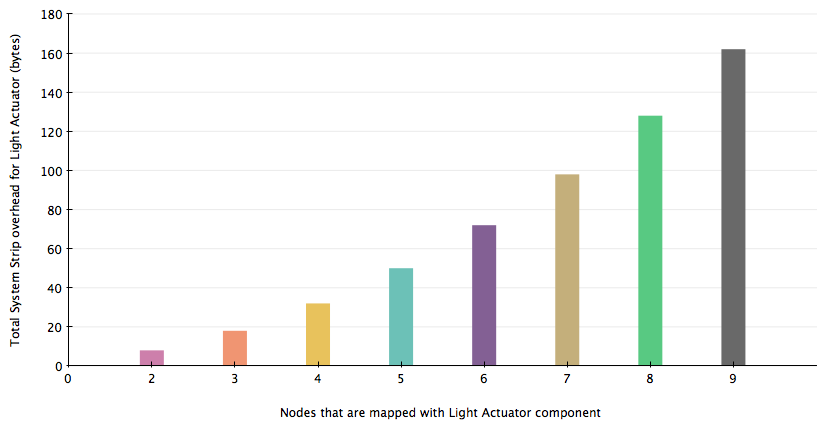
\includegraphics[width=\linewidth]{figures/results-system-overhead-vs-network-size}
\caption{The total memory overhead of a Light Actuator strip aggregated among its members at different member size}
\label{fig:results-system-overhead-vs-network-size}
\end{figure}

%\begin{figure}[h!]
%\centering
    %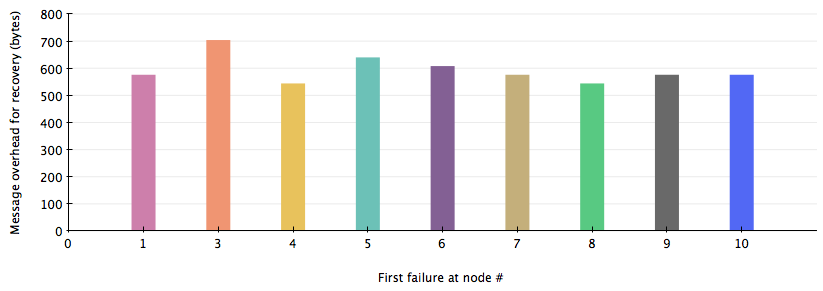
\includegraphics[width=\linewidth]{figures/results-message-overhead}
%\caption{Message overhead used to recover for node as first failure}
%\label{fig:results-message-overhead}
%\end{figure}

\begin{figure}[h!]
\centering
    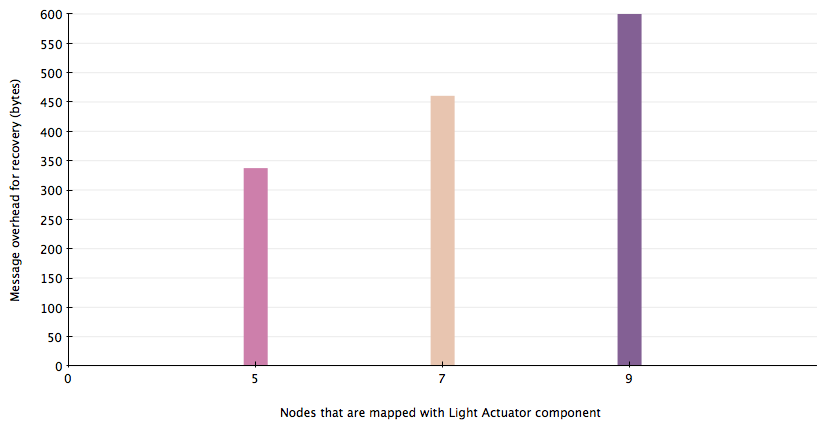
\includegraphics[width=\linewidth]{figures/results-message-overhead-vs-strip-size}
\caption{Message overhead for recovery of a random Light Actuator strip member failure against dfferent strip sizes}
\label{fig:results-message-overhead-vs-strip-size}
\end{figure}

\begin{figure}[h!]
\centering
    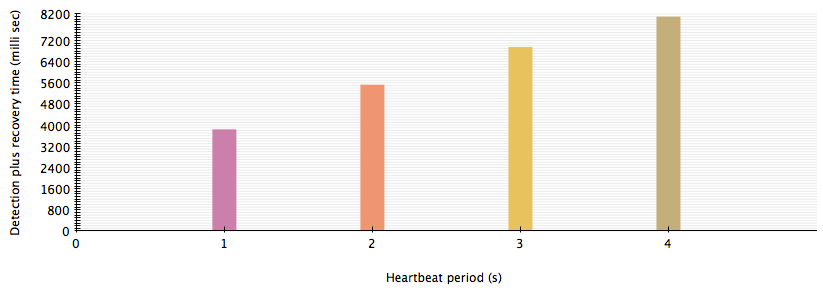
\includegraphics[width=\linewidth]{figures/results-heartbeat-vs-detection-recovery-time}
\caption{Detection plus recovery time in milli-seconds for heartbeat period in seconds}
\label{fig:results-heartbeat-vs-detection-recovery-time}
\end{figure}

\begin{figure}[h!]
\centering
    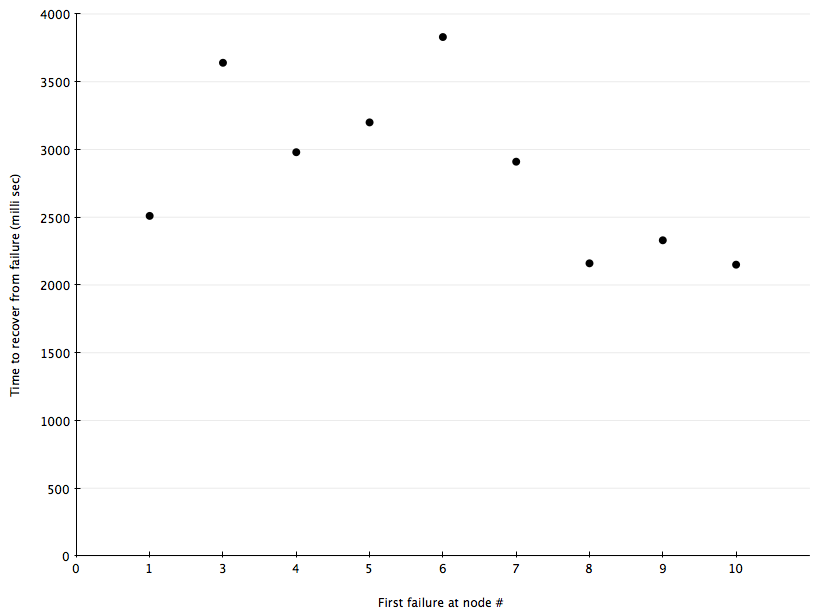
\includegraphics[width=\linewidth]{figures/results-average-recovery-time-plus-message-overhead}
\caption{Average recovery time over 5 deployments for each node failure as the first failure}
\label{fig:results}
\end{figure}

